\documentclass[../thesis.tex]{subfiles}

\begin{document}

In this chapter, we present an alternative end-to-end controller that maps the multi-sensor input directly to the action space based on deep reinforcement learning (DRL), a recently very popular research field. 
We propose two novel methods that effectively train the multimodal sensor policy without over-fitting to partial sensor subset, namely \textit{Sensor Dropout} and \textit{Auxiliary Loss}. 
Two popular continuous action DRL algorithms namely Normalized Advantage Function (NAF) \cite{CDQN} and Deep Deterministic Policy Gradient (DDPG) \cite{DBLP:journals/corr/LillicrapHPHETS15}, are picked and augmented to accept multi-modal input. The resulting autonomous navigation policy is tested exhaustively to verify its performance in a physics-based gaming environment called TORCS \cite{wymann2000torcs}. 

Through extensive empirical testing we show the following exciting results,
\begin{enumerate}

	\item Multimodal-DRL with Sensor Dropout(SD) reduces performance drop in a noisy environment from $\approx 40\%$ to just $10\%$, when compared to a baseline single sensor system.
	
	\item Policies learned using SD best leverage the multi-modal setting by greatly reducing over-dependence on any one sensing modality. Additionally, for each sensor it was observed that SD enforces sparsity and promotes each sensor to base the policy primarily on intuitive and salient features.
	
	\item A multi-modal policy with SD guarantees functionality even in a face a sensor failure. This is a huge plus and the best use-case for the need for redundancy in safety-critical application like autonomous navigation.

\end{enumerate}


The chapter is organized as follows: 
% Section \ref{sec:mdrl-background} summarizes the background of DRL and two DRL algorithms we extended in this work. 
Section \ref{sec:mdrl-proposed} introduces two methods on effectively training a multimodal sensor policy. We first introduce a new stochastic regularization called Sensor Dropout, and details its advantages over the standard Dropout for this problem. The resulting policy can be further fine tuned by adding additional auxiliary losses to reduce the action variance. The performance of Sensor Dropout is then validated in Section \ref{sec:mdrl-results}. In Section \ref{sec:mdrl-discussion}, we summarize our results and discuss key insights obtained through this exercise. 
% Finally, Section 6 contains conclusions and ideas for future work. 


\section{Proposed Methods} \label{sec:mdrl-proposed}

% \subsection{Motivation} 
Multi-modal DRL aims to leverage the availability of multiple, potentially imperfect, sensor inputs to improve learned policy. Most autonomous driving vehicles have been equipped with an array of sensors like GPS, Lidar, Camera, and Odometer, etc \cite{hudda2013self}. While one would offer a long range noisy estimate, the other would offer a shorter range accurate one. When combined though, the resulting observer will have a good and reliable estimate of the environment. This problem is critical as a further step toward the real-world robotics application given the current state-of-the-art DRL agents on many realistic simulators. 


\subsection{Multi-modal Network Architecture}

% Feature Extraction Module %

We denote a set of observations composed from $M$ sensors as, $S = [S^{(1)}~S^{(2)}~..~S^{(M)}]^T$, where $S^{(i)}$ stands for observation from $i^{th}$ sensor. In the multi-modal network, each sensory signal is pre-processed along independent paths. Each path has a feature extraction module with an appropriate network architecture, using randomly initialized or pre-trained weights. In this work, we use three different inputs namely image, laser scan and physical parameters (like wheel speed, position, odometry, etc. The details of each of the feature extraction module are listed in the Appendix. The modularized feature extraction stages for multiple inputs naturally allows for independent extraction of salient information that is transferable (with some tuning if needed) to other applications like collision avoidance, pedestrian detection and tracking, etc. The schematic illustration of modularized Multi-modal architecture is shown in Fig. \ref{fig:Multi-SD}. The outputs of feature extraction modules are eventually flattened and concatenated to form the multi-modal state. 

\subsection{Sensor-based Dropout (SD)} \label{sec:SD}

\begin{figure}[t]
	\begin{center}
	\centerline{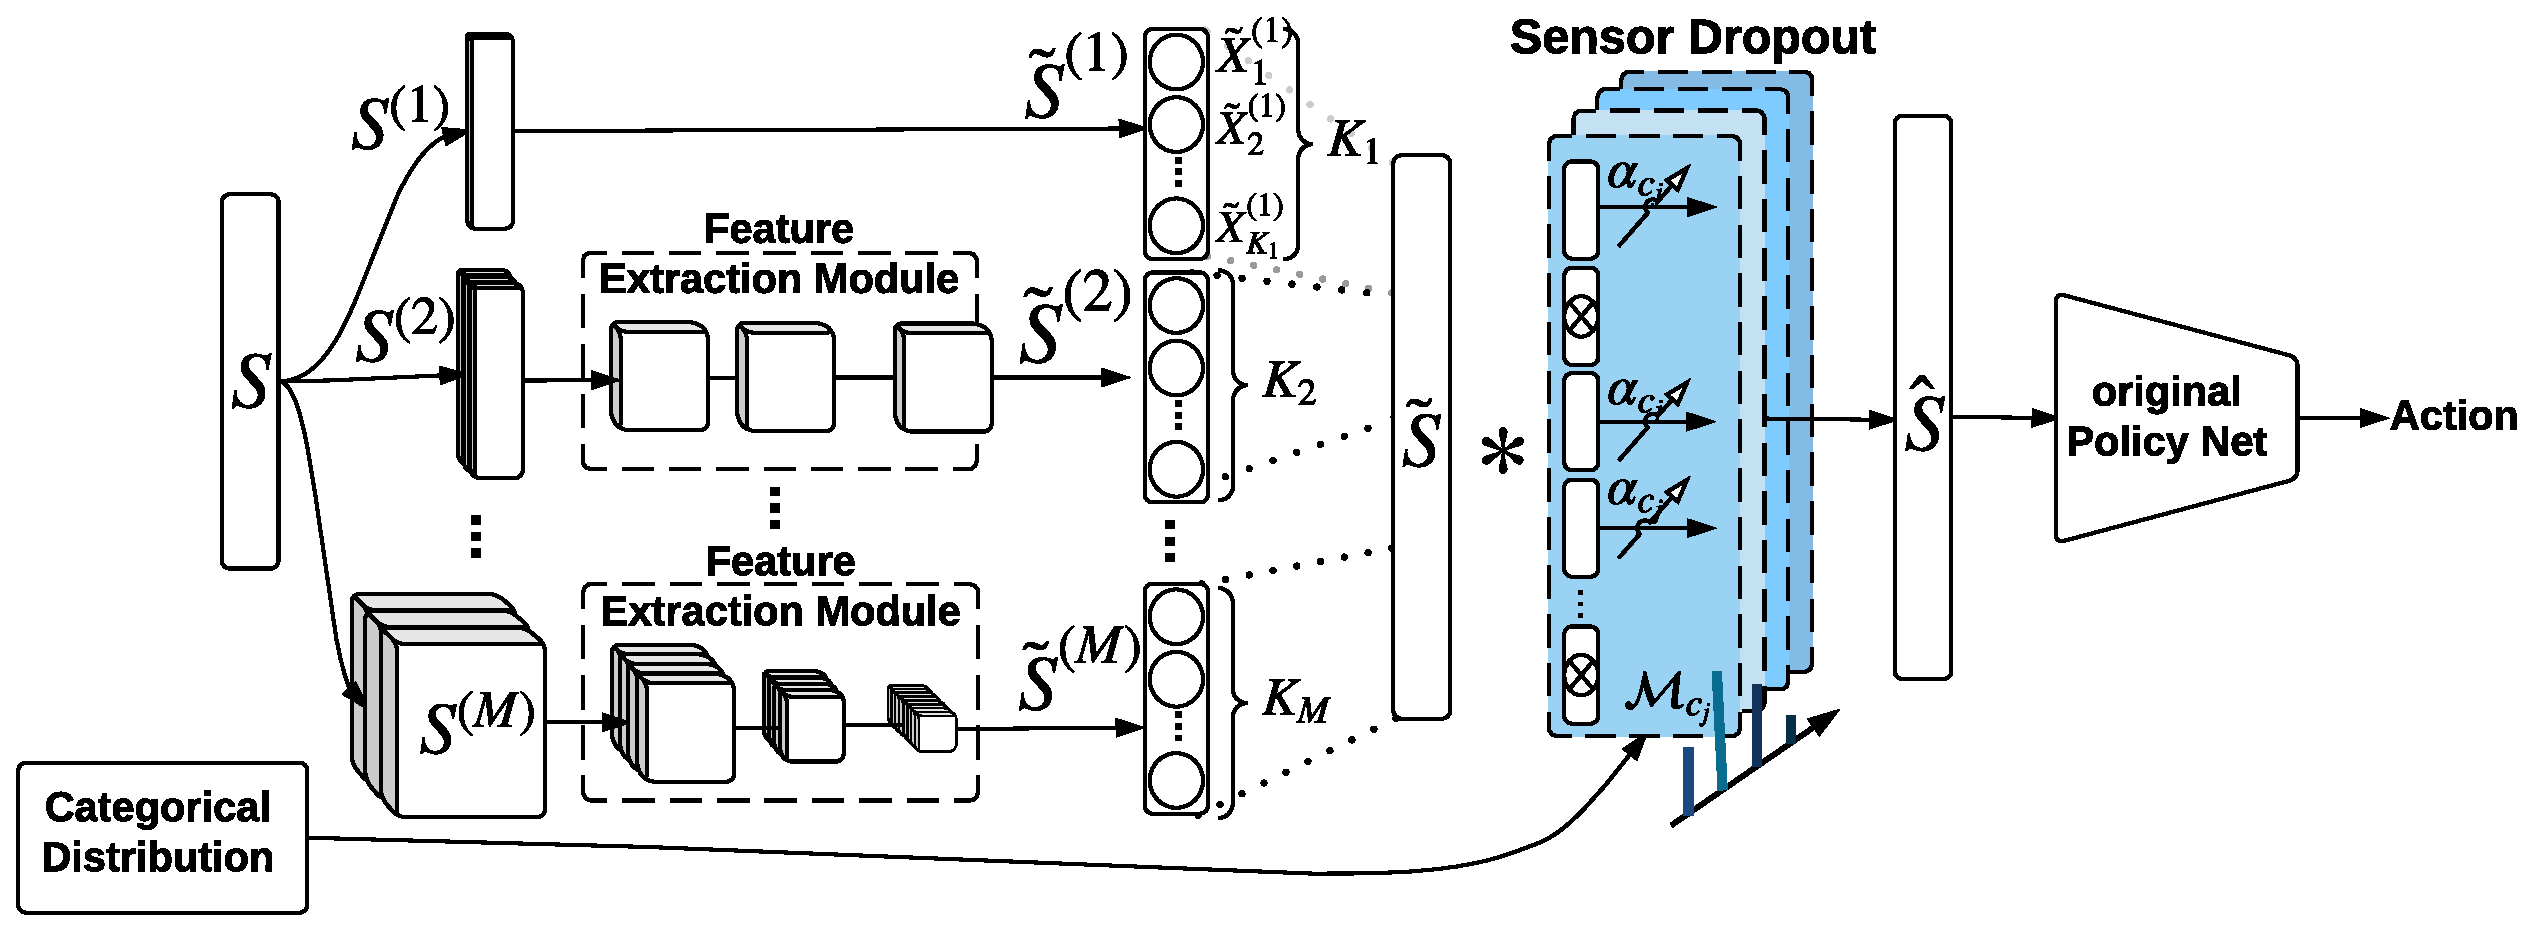
\includegraphics[width=0.8\columnwidth]{./MultimodalDRL/fig/SD_new}} % sd
	\caption{Illustration of multimodal sensor policy network augmented with Sensor Dropout. The operation $*$ stands for element-wised multiplication. The dropping configuration of Sensor Dropout is sampled from a categorical distribution, which the network takes as an additional input. The feature extraction module can be either pure identity function (modality $1$), or convolution-based layer (modality $2 \to M$). The operation $*$ stands for element-wised multiplication.}
	\label{fig:Multi-SD}
	\end{center}
\end{figure} 


The Sensor Dropout (SD) is a variant of the vanilla Dropout \cite{dropout} that maintains dropping configurations on each sensor module instead of individual neuron. Though both methods share a similar motivation on stochastic regularization, SD is more better-motivated for training the multimodal sensor policy. By randomly dropping the sensor block during training, the policy network is encouraged to exploit the modularized structure among each sensor stream. In the application to the complex robotics system, SD has advantages on handling imperfect conditions such as latency, noises, and even partial sensor failure.

% The resulting multimodal policy has a nice property that it can perform even in the absence of partial sensor modalities, as long as at least one is fully functioning. 

As shown in Fig.\ref{fig:Multi-SD}, consider the multimodal state $\tilde{S}$, obtained from feature extraction and given by $\tilde{S}=[\tilde{S}^{(1)}~\tilde{S}^{(2)}~..~\tilde{S}^{(M)}]^T$, where $\tilde{S}^{(i)}= [\tilde{X}_1^{(i)}~\tilde{X}_2^{(i)}~..~\tilde{X}_{K_i}^{(i)}]^T$. 
The dropping configuration is defined as a $M$-dimensional vector $\mathbf{c} = [\delta_{c}^{(1)}~\delta_{c}^{(2)}~..~\delta_{c}^{(M)}]^T$, where each element $\delta_{c}^{(i)} \in \{0,1\}$ represents the on/off indicator for the $i^{th}$ sensor modality. We now detail the two main differences between original Dropout and SD along with their interpretations. 

% 1. Categorical Distribution
Firstly, note that the dimension of the dropping vector $\mathbf{c}$ is much lower than the one in the standard Dropout ($\sum_{i=1}^M K_i$). As a consequence, the probability of the event where all sensors are dropped out (i.e. $\mathbf{{c_0}} = [0^{(1)}~0^{(2)}~..~0^{(M)}]^T$) is not negligible in SD. To explicitly remove $\mathbf{{c_0}}$, we slightly depart from \cite{dropout} in modeling the SD layer. Instead of modeling SD as random process where any sensor block $\tilde{S}^{(i)}$ is switched on/off with a \textit{fixed} probability $p$, we define the random variable as the dropping configuration $\mathbf{c}$ itself. Since there are $N = 2^M - 1$ possible states for $\mathbf{c}$, we accordingly sample from an $N$-state categorical distribution $\mathbb{P}$. The categorical distribution not only offers convenience in analysis and interpretation over standard Bernoulli on sensor blocks, but is better-motivated in that it can be adaptive to the current sensor reliability during run-time. We denote the probability of a dropping configuration $\mathbf{{c_j}}$ occurring with $p_j$, where the subscript $j$ ranges from $1$ to $N$. The corresponding pseudo-Bernoulli
\footnote{ 
We wish to point out that $p^{(i)}$ is pseudo-Bernoulli as we restrict our attention to cases where at least one sensor block is switched on at any given instant in the layer. This implies that, while the switching on of any sensor block $\tilde{S}^{(i)}$ is independent of the other, switching off is not. So the distribution is no longer fully independent.
}
distribution for switching on a sensor block $\tilde{S}^{(i)}$ can be calculated as $p^{(i)} = \sum_{j=1}^N\delta_{c_j}^{(i)} p_j$. 


% 2. Rescaling Process
Another difference from the standard Dropout is the rescaling process. Unlike the standard Dropout which preserves a \textit{fix} scaling ratio after dropping neurons, the rescaling ratio in SD is formulated as a function of the dropping configuration and sensor dimensions instead. The intuition is to keep the weighted summations equivalent among different dropping configurations in order to activate the later hidden layers. The scaling ratio is calculated as $\alpha_{c_j} = \frac{\sum_{i=1}^M K_i }{\sum_{i=1}^M \delta_{c_j}^{(i)} K_i}.$ In summary, the output of SD for the $k^{th}$ feature in $i^{th}$ sensor block (i.e. $\tilde{S}^{(i)}$) given a dropping configuration $\mathbf{c_j}$ can be shown as,
\begin{align}
\hat{S}^{(i)}_{{c_j},k} &= \mathcal{M}^{(i)}_{c_j} \tilde{X}_k^{(i)}, \ 
&\text{where} \ \mathcal{M}^{(i)}_{c_j} = \alpha_{c_j} \delta_{c_j}^{(i)}. 
\end{align}
$\mathcal{M}^{(k)}_{c_j}$ is an augmented mask encapsulating both dropout and re-scaling. 
 
\subsection{Augmenting Auxiliary Loss}

An alternative interpretation of the SD-augmented policy is that sub-policy induced by each sensor combination are jointly optimized during training. Denote the ultimate policy and sub-policy induced by each sensor combination as $\mu_{\mathbf{c}\sim \mathbb{P}}$ and $\mu_{c_j}$, respectively. The final output maintains a geometric mean over $N$ different actions. 

Despite the expectation of the total policy gradients for each sub-policy is the same, SD provides no guarantees on the consistency of these actions. 
To encourage the policy network to extract salient features from each sensor that can be embedded with similar representation in the policy network, we further augment an auxiliary loss that penalizes the inconsistency among $\mu_{c_j}$. 
This additional penalty term provides an alternative gradient that reduces the variation of the ultimate polciy, i.e. $Var \left[ \mu_{\mathbf{c}\sim \mathbb{P}} \right]$.
% In fact, policy gradients point the sub-policy toward maximum value state yet has no guarantees on the consistency provides only the (noisy) direction toward In fact, if the environment provides only sparse reward signal, the sub-policy is trained 
% To encourage the policy network to extract salient features from each sensor that \textit{share} representative information for decision making, we augment an auxiliary loss that penalizes the inconsistency among $\mu_{c_j}$. 

The mechanism is motivated from the recent successes \cite{DBLP:journals/corr/GuLGTL16,mirowski2017a,lample2016playing,dosovitskiy2016learning} that exploit how adding the auxiliary tasks help greatly improve both agent's performance and convergence rate. However, unlike most previous works that pick up the auxiliary tasks carefully from the ground truth environment, we formulate the \textit{target action} from the policy network itself. 
Under the standard actor-critic architecture, the target action is defined as the sub-policy $\tilde{\mu}_{c^{*}}$ among target actor network $\tilde{\mu}_{\mathbf{c}\sim \mathbb{P}}$ that maximize the the target critic values $\tilde{Q}$.
\begin{align}
L_{aux} &= \lambda \sum_{i=1}^N (\mu_{c_j}(s_i)-\tilde{\mu}_{c^{*}}(s_i))^2 \\
\text{where  } c^{*} &= \mathop{\mathrm{argmax}}_{c_j \sim \mathbb{P}} \sum_{i=1}^N \tilde{Q}(s_i,\tilde{\mu}_{c_j}(s_i))
\end{align}

% \begin{align}
% L_{aux} &= \lambda \frac{1}{N} \sum_{i=1}^N (\mu_{c_j}(s_i)-\tilde{\mu}^{*}(s_i))^2 \\
% \mu^{*} &= \mathop{\mathrm{argmax}}_{\mu \in \left \{ \mu_{c_j} \right \} \text{, where} c_j \sim \mathbb{P}} \frac{1}{N} \sum_{i=1}^N Q(s_i,\mu(s_i))
% \end{align}
% $\tilde{\mu}$ and $\tilde{Q}$ represent the target actor and target critic network that maintain an exponentially moving average to stabilize training. 
Here, $\lambda$ is an additional hyperparameter that indicates the importance ratio between the two losses, and $N$ is the batch size for off-policy learning.

% The derived auxiliary loss therefore preserves a temporal-difference (TD) method that \textit{learn a guess from a guess} \cite{}. 

% it is possible that actions suggested by each policy varies a lot. 



\section{Evaluation and Analysis} \label{sec:mdrl-results}
In this section, we outline our experimental setup using TORCS simulator and then exhaustively compare the performance of the trained policies on both DDPG and NAF algorithms with and without Sensor Dropout. The exhaustive analysis includes policy robustness, sensitivity, and dependency on each sensor modality. Finally, we use a perturbation-based technique to visualize the learned policies and finally discuss some of the interesting findings of this exercise.

\subsection{Platform Setup} \label{sec:platform}

\begin{figure}[t]
	\centering
	\vskip 0.2in
	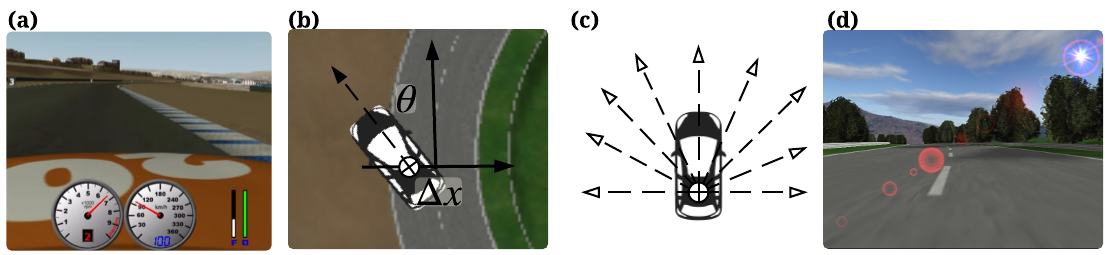
\includegraphics[width=\columnwidth]{./MultimodalDRL/fig/TORCS.png} % torcs.png
	\caption{Sensors used in the TORCS racing car simulator: \textit{Sensor 1:} Physical information such as velocity (a), position, and orientation (b), \textit{Sensor 2:} Laser range finder (c), and \textit{Sensor 3:} Front-view camera (d).}
	\label{fig:TORCS}
\end{figure} 

\textbf{TORCS Simulator}
The proposed approach was verified on TORCS \cite{wymann2000torcs}, a popular open-source car racing simulator that is capable of simulating physically realistic vehicle dynamics as well as multiple sensing modalities \cite{GymTORCS} to build sophisticated AI agents. In order to make the learning problem representative of the real-world setting, we picked the following sensors from the TORCS package: the 2D laser range finder, front-view camera with RGB channel, vehicle state - position and speed. The action space is a continuous vector in $\mathbb{R}^2$, whose elements represent steering angle, and acceleration. 

As shown in Fig. \ref{fig:TORCS}, the physical state is a $10$ DOF hybrid state, including $3$D velocity ($3$ DOF), position and orientation with respect to track center-line ($2$ DOF), and finally rotational speed of $4$ wheels ($4$ DOF) and engine ($1$ DOF). Each laser scan is composed of $19$ readings spanning a $180\degree$ field-of-view in the the front of car. Finally, camera provides RGB channels with resolution $64 \times 64$. We use the following sensing modalities for our state description: (1) We define \emph{Sensor 1} as a hybrid state containing physical-based information such as odometry and simulated GPS signal. (2) \emph{Sensor 2} consists of $4$ consecutive laser scans (i.e., at time $t$, we input scans from times $t,~ t-1,~t-2~\&~t-3$). Finally, as \emph{Sensor 3}, we supply $4$ consecutive color images capturing the car's front-view. These three representations are used separately to develop our baseline uni-modal sensor policies. The multi-modal state on the other hand has access to all sensors at any given point. When Sensor Dropout (SD) is applied, agent will randomly lose access to a strict subset of sensors. The categorical distribution is initialized with a uniform distribution among total $7$ possible combinations of sensor subset, and the best learned policy is reported here. 

An exploration strategy is injected adding an Ornstein-Uhlenbeck process noise \cite{uhlenbeck1930theory} to the output of the policy network. The choice of reward function is slightly different from  \citet{DBLP:journals/corr/LillicrapHPHETS15} and \citet{A3C} as an additional penalty term to penalize side-ways drifting along the track was added. In practice, this modification leads to more stable policies during training \cite{BenLau16}. 

\textbf{Network Architecture}
For laser feature extraction module, we use two $1D$ convolution layers with $4$ filters of size $4 \times 1$, while image feature extraction is composed of three $2D$ convolution layers: one layer of $16$ filters of size $4 \times 4$ and striding length $4$, followed by two layers each with $32$ filters of size $2 \times 2 $ and striding length $2$. Batch normalization is followed after every convolution layer. All these extraction modules are fused and are later followed up with two fully-connected layers of $200$ hidden units each. All hidden layers have \emph{relu} activations. The final layer of the critic network use \emph{leaner} activation, while the output of the actor network are bounded using \emph{tanh} activation. We use sigmoid activation for the output of $L$ network in NAF. In practice, it leads to a more stable training for high dimensional state space. We trained with minibatch size of $16$. 

We used Adam \cite{adam} for learning the network parameters. For DDPG, the learning rates for actor and critic are $10^{-4}$ and $10^{-3}$, respectively. We allow the actor and critic to maintain its own feature extraction module. In practice, sharing the same extraction module can lead to unstable training. Note that the NAF algorithm maintains three separate networks, which represent the value function ($V(s|\theta^V)$), policy network ($\mu(s|\theta^\mu)$), and the state-dependent covariance matrix in the action space ($P(s|\theta^L)$), respectively. In order to maintain a similar experiment setting and avoid unstable training, we maintain two independent feature extraction modules for $\theta^\mu$, and both $\theta^V$ and $\theta^L$. In a similar vein, we apply a learning rate of $10^{-4}$ for $\theta^\mu$, and $10^{-3}$ for both  $\theta^\mu$ and $\theta^V$. 

\begin{table}[t]
    \vskip 0.1in
    \caption{Model Specification}
    \label{table:model-spec}
    \vskip 0.1in
    \centering
    \begin{small}
%     \begin{sc}
    \begin{tabular}{ccc}
    \toprule 
    \centering
    Model ID & State Dimensionality & Description \\ \midrule \midrule
    Physical & 10 & \\
    Lasers & 4 $\times$ 19 & 4 consecutive laser scans \\
    Images & 12 $\times$ 64 $\times$ 64 & 4 consecutive RGB image \\
    Multi  & 10+1$\times$19+3$\times$64$\times$64 & all sensor streams at current time step \\ \toprule
    \end{tabular}
%     \end{sc}
    \end{small}
\end{table}


\subsection{Experimental Results} % FIXME start from here
\subsubsection{Training Summary}

\begin{figure}[t]
    \centering
    \begin{subfigure}[b]{0.48\linewidth}
        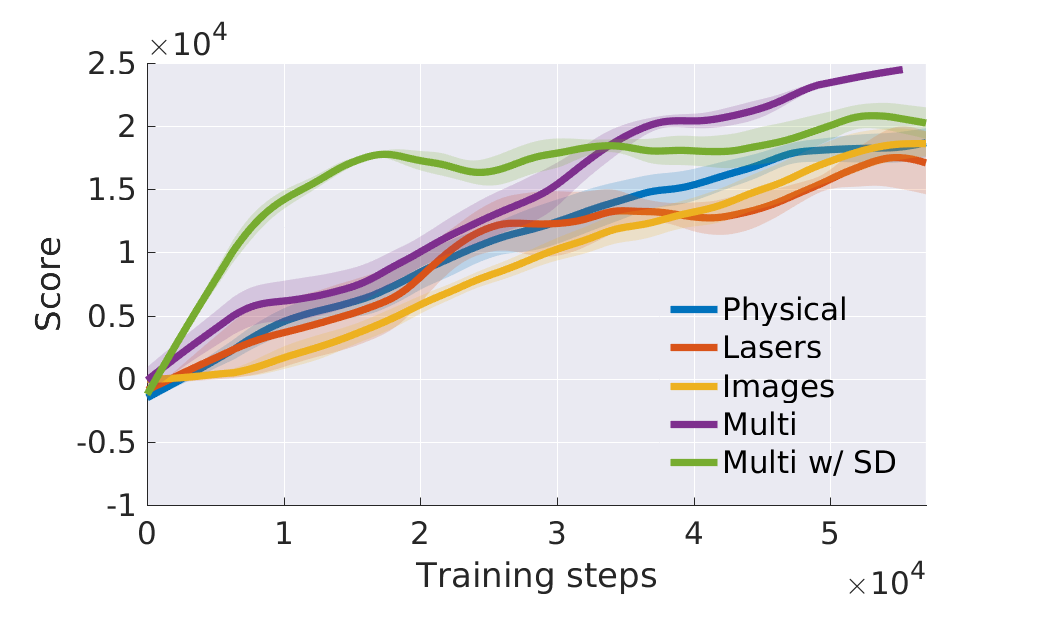
\includegraphics[width=\columnwidth]{./MultimodalDRL/fig/training_step_naf_without_aux}
        \subcaption{NAF}
        \label{fig:training_exp_naf}
    \end{subfigure}
    \begin{subfigure}[b]{0.48\linewidth}
        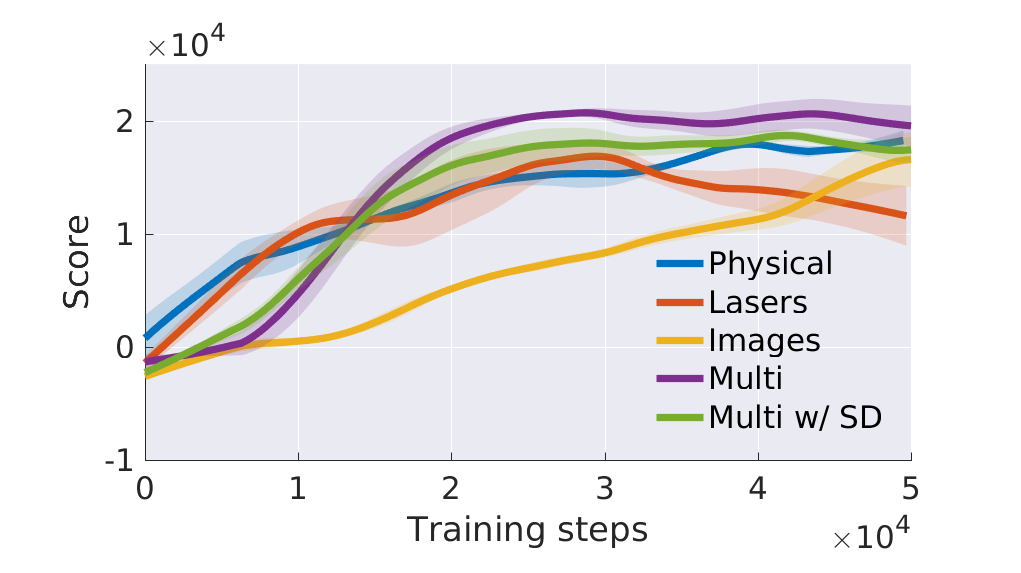
\includegraphics[width=\columnwidth]{./MultimodalDRL/fig/training_step_ddpg_without_aux}
        \subcaption{DDPG}
        \label{fig:training_exp_ddpg}
    \end{subfigure}
    \caption{Training performance comparison of three baseline single sensor policies, and the proposed multi-modal policies, with and without Sensor Dropout.}
    \label{fig:training_exp}
\end{figure}

% \textbf{Training Summary:}
The training performance, for all the proposed models and their corresponding baselines, is shown in Fig. \ref{fig:training_exp}. The blue, red, and orange line represents three uni-modal policies. 
For DDPG, using high dimensional sensory input directly impacts convergence rate of the policy. (Note that the \textit{Images} uni-policy has a much larger dimensional state space compared with \textit{Multi} policy.) 
Counter-intuitively, NAF performs a nearly linear improvement over training steps, and is relatively insensitive to the dimensionality of the state space. However, adding Sensor Dropout (SD) dramatically increases the convergence rate.
Note that for both algorithms, the final performance for multimodal sensor policies trained with SD is slightly lower than training without SD, indicating that SD has a stochastic regularization effect similar to original Dropout.
% We denote the difference of the performance to the fundamental formulation of the value-based method (NAF) and actor-critic method (DDPG). 


\subsubsection{Comparison with Baseline Models}

\begin{figure}[t]
    \centering
    \begin{subfigure}[b]{0.48\linewidth}
        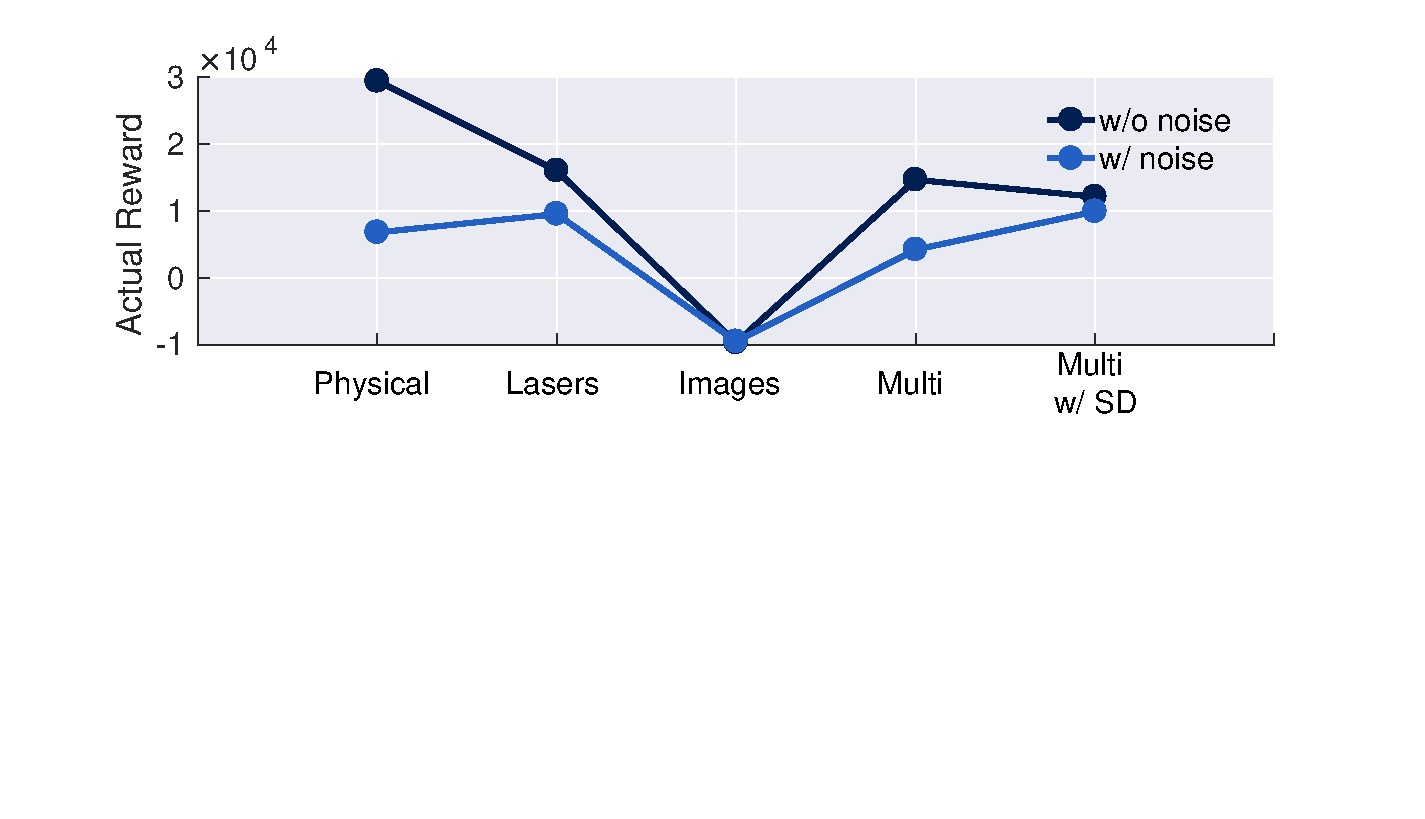
\includegraphics[width=\columnwidth,trim= 45 180 45 10, clip=true]{./MultimodalDRL/fig/actual_robust_naf}
        \subcaption{NAF}
        \label{fig:actual_robust_naf}
    \end{subfigure}
    \begin{subfigure}[b]{0.48\linewidth}
        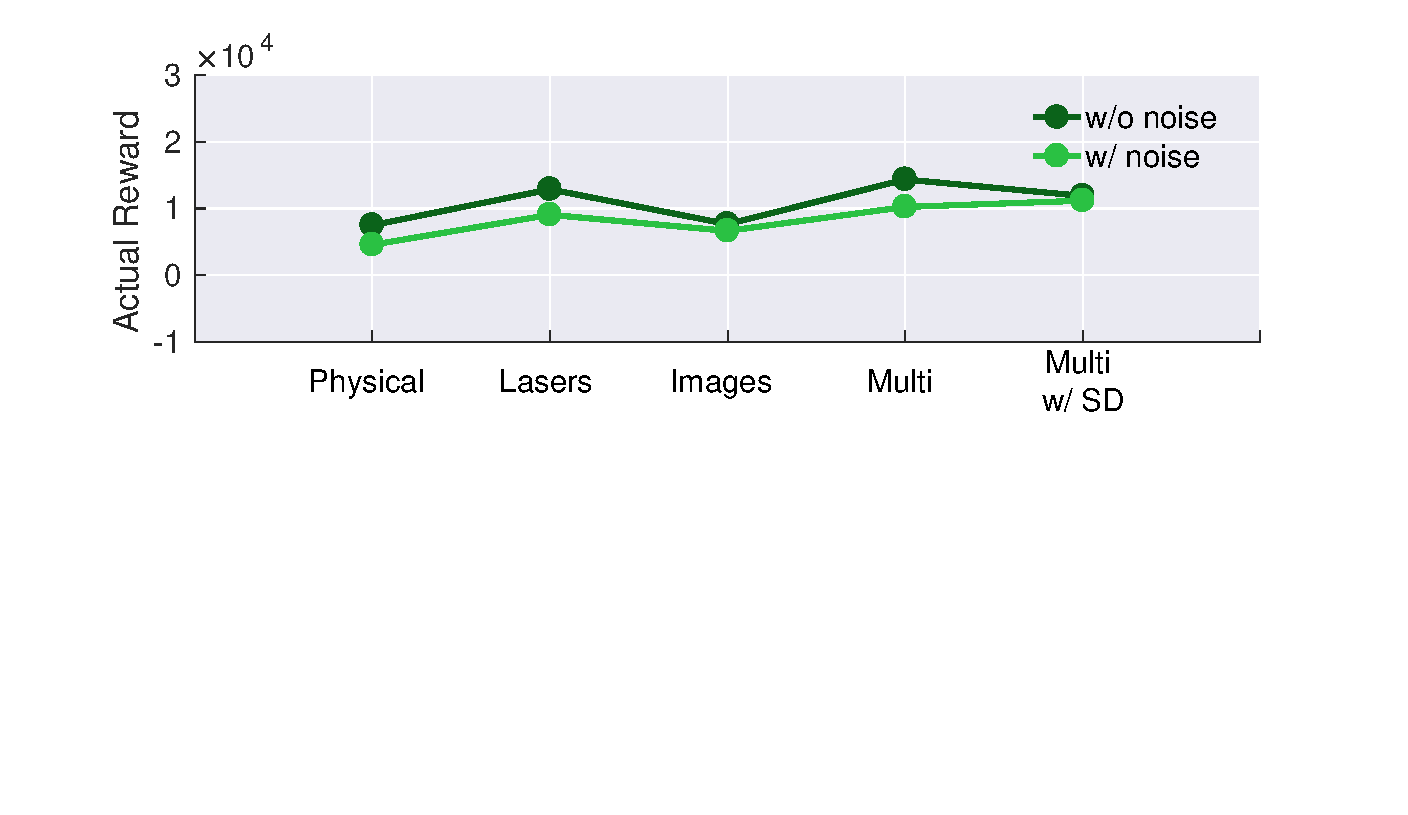
\includegraphics[width=\columnwidth,trim= 45 180 45 10, clip=true]{./MultimodalDRL/fig/actual_robust_ddpg}
        \subcaption{DDPG}
        \label{fig:actual_robust_ddpg}
    \end{subfigure}
    \caption{Policy Robustness Analysis: Darker lines connects average rewards of leaned policies with accurate sensing while the lighter lines connects the corresponding policies in the face of sensor noise.}
    \label{fig:actual_robust}
\end{figure}

\begin{figure}[t]
    \centering
    \begin{subfigure}[b]{0.48\linewidth}
        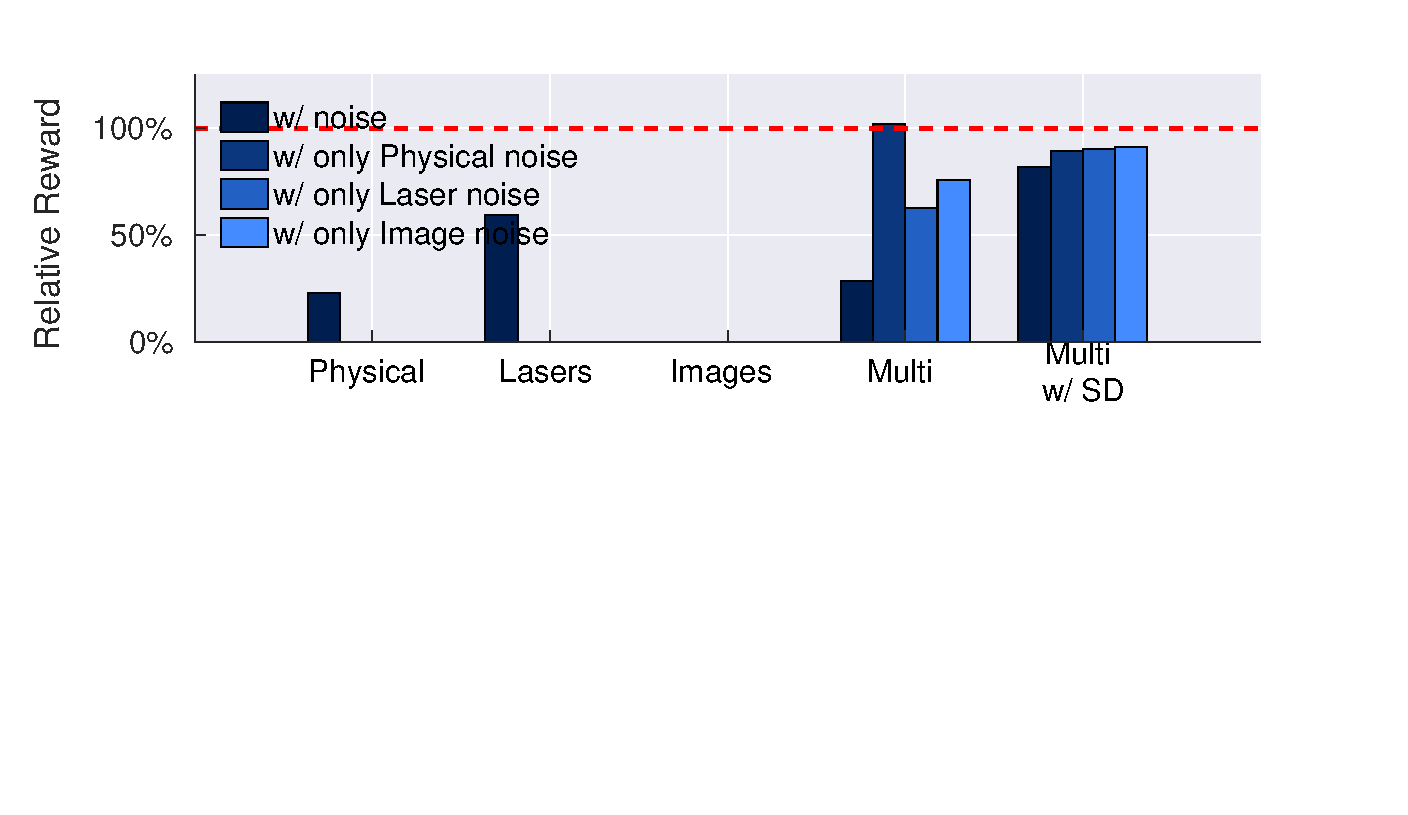
\includegraphics[width=\columnwidth,trim= 45 180 45 25, clip=true]{./MultimodalDRL/fig/relative_robust_naf}
        \subcaption{NAF}
        \label{fig:relative_robust_naf}
    \end{subfigure}
    \begin{subfigure}[b]{0.48\linewidth}
        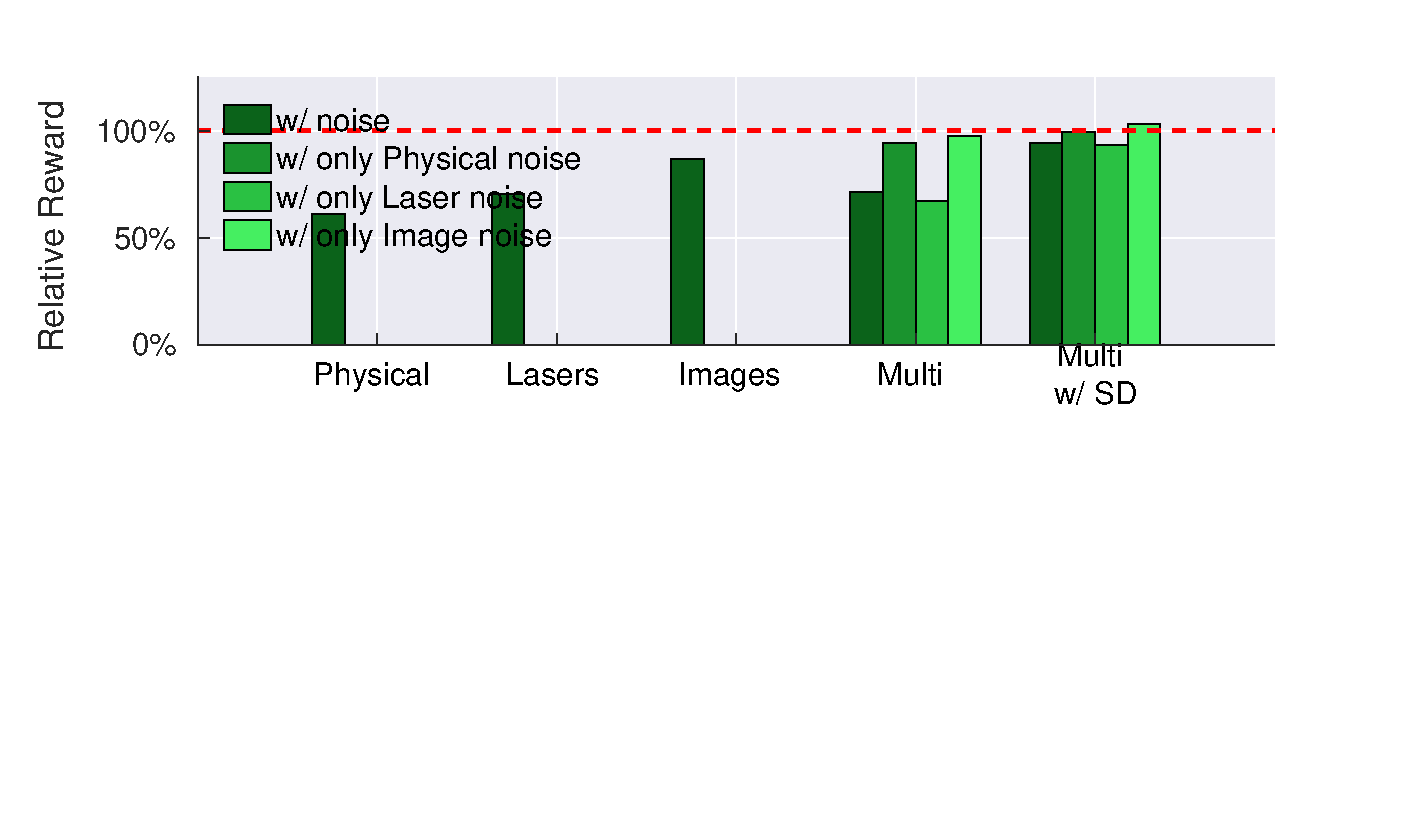
\includegraphics[width=\columnwidth,trim= 45 180 45 25, clip=true]{./MultimodalDRL/fig/relative_robust_ddpg}
        \subcaption{DDPG}
        \label{fig:relative_robust_ddpg}
    \end{subfigure}
    \caption{Policy Robustness Analysis: The bar box measures the relative scale among each of the models when noise is introduced. The red dotted lines show the performance without noise.}
    \label{fig:relative_robust}
\end{figure}

\textbf{Uni-modal policies:} 
Note that, we assume perfect sensing during the training. However, to test performance in a more realistic scenario, we simulate mildly imperfect sensing by adding gaussian noise. The perturbation sensitivity is compatible with a more standard Average Fisher Sensitivity (AFS) according to \cite{progressive_net}. Policy performance with and without noise is plotted for comparison in Fig. \ref{fig:actual_robust} and \ref{fig:relative_robust}. While Fig. \ref{fig:actual_robust} plots the actual reward performance, Fig. \ref{fig:relative_robust} summarizes the relative performance compared with a noiseless environment. 

The performance of the NAF agent drops dramatically when the noise is introduced. We also observe that NAF in the multi-modal is sensitive to states from sensors which are easily interpretable such as laser scanners. This effect shows that using an over-complete state representation holds a risk of the agent learning an undesired policy where the influence of different features gets unbalanced. The regularization introduced by Sensor Dropout alleviates this issue and learns a stable policy on both algorithms, with only slight decrease of the performance compared with multi-modal agents trained without SD. In summary, with the addition of noise the performance drop is sometimes severe in a single input policy, as seen for NAF with physical state input. In comparison, the drop is ore contained for the multi-modal policy and almost negligible when Sensor Dropout is used.


\begin{table}[t]
    \vskip 0.1in
    \caption{Performance of Policy }
    \label{table:multiple-uni-baseline}
    \vskip 0.1in
    \centering
    \begin{small}
    \begin{sc}
    \begin{tabular}{c|cc|c}
    \toprule 
    \centering
    Policy & w/o Noise & w/ Noise & Performance Drop \\ \midrule \midrule
     Multi Uni-modal w/ Meta Controller & 1.51 $\pm$ 0.57 & 0.73 $\pm$ 0.40 & 51.7 \% \\
     Multimodal w/ SD & 2.54 $\pm$ 0.08 & 2.29 $\pm$ 0.60 & 9.8 \% \\ \toprule
    \end{tabular}
    \end{sc}
    \end{small}
\end{table}

\textbf{Multiple Uni-modal Policy:}
Another intuitive baseline for the multi-sensor problem is to train each uni-modal sensor policy separately. Once individual policies are learned, we can train an additional meta controller that select which policy to follow given the current state.
For this, we take the best trained policies of each sensor, and train a meta controller that takes the concatenated feature state from each sensor and output a $3 DOF$ softmax layer as the probability of choosing each uni-modal sensor policy. The meta controller is trained under the standard policy gradient method, which can be found in \cite{meta_policy} for more details.

Policy performance with and without noise for two approaches are summarized in Table \ref{table:multiple-uni-baseline}. 
The performance of the baseline policy drops dramatically once noise is introduced, which implies that without any regularization the uni-modal policy is prone to overfit. In fact, with the addition of noise the performance drop is sometimes severe in physical-based or laser-based policy. 
% We also suspect it is because of the inconsistency of actions when switching among different uni-modal policies. 
In comparison, the policy trained with SD reaches a higher score in both scenarios, and the drop is almost negligible.
 
% While the image-based policy is usually more aggressive as it can foresee a longer horizon, the physical-based or laser-based policy drives more cautiously. 



% B. Without Noise experiment % 
% 1. DDPG looks well
% 2. Uni-modal NAF : actual reward decrease proportionally when state dim. increase or state is too abstract.
% -> we claim Multi-modal setting help alleviate the situation
% C. With Noise experiment % 
% 1. NAF perform poorly when noise is introduced. DDPG on the other hand is less sensitive to noise 2. Introducing of SD help both algorithm 


\subsubsection{Policy Robustness Analysis}
% \label{sec:policy}

\begin{table}[t]
  \begin{minipage}[t]{0.45\linewidth}
    \centering
    \vskip -0.1in
    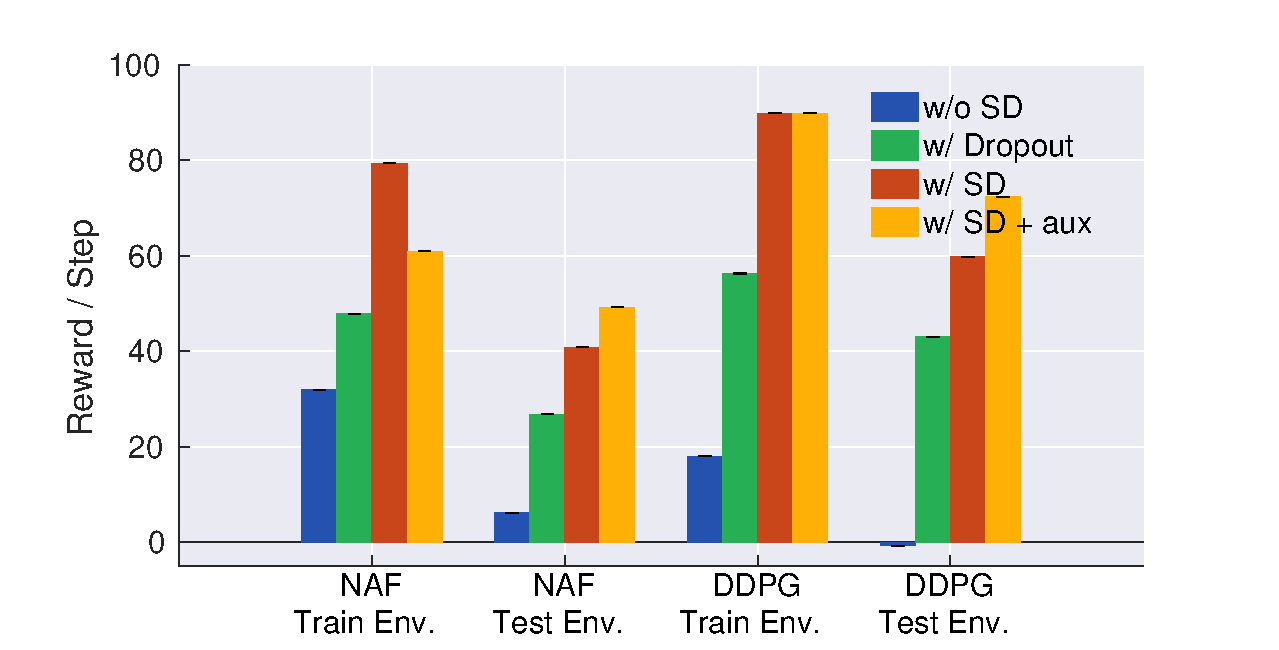
\includegraphics[width=\columnwidth]{./MultimodalDRL/fig/random_sensor_failure_normalize_with_aux}
%     \vskip 0.05in
    \captionof{figure}{Policy performance when facing random sensor failure.}
    \label{fig:random_sensor_failure}
  \end{minipage}
  \begin{minipage}[t]{0.45\linewidth}
    \vskip -0.1in
    \caption{Results of the sensitivity metric.} % $\mathcal{T}_2^1$
    \label{table:policy-ratio}
    \vskip 0.1in
    \centering
    \begin{small}
    \begin{sc}
    \begin{tabular}{cccc}
    \toprule 
    \centering
     & & Training & Testing  \\ 
     & & Env. & Env. \\ \midrule \midrule
    \multirow{2}{*}{NAF}  & w/o SD & 1.651 & 1.722 \\
                          & w/ SD  & \textbf{1.284} & \textbf{1.086} \\ \midrule
    \multirow{2}{*}{DDPG} & w/o SD & 1.458 & 1.468 \\
                          & w/ SD  & \textbf{1.168} & \textbf{1.171} \\ \toprule
    \end{tabular}
    \end{sc}
    \end{small}
  \end{minipage}
\end{table}

% \textbf{Policy Robustness Analysis:}
In this part, we further validate our hypothesis that SD reduces the learned policy's acute dependence on a subset of sensors in a multi-modal setting. First, we considered a scenario when malfunction of a sensor has been detected by the system, and the agent need to rely on the remaining sensors to make the decision. During testing, we randomly blocked off part of the sensor modules, and scaled the rest of observation using the same rescaling mechanism as proposed in Section \ref{sec:SD}. Fig. \ref{fig:random_sensor_failure} reports the average of the normalized reward of each model. A naive multimodal policy without any stochastic regularization (blue bar) performs poorly in the face of partial sensor failure and transfer tasks. Adding original Dropout does make the policy more generalized, yet the performance is not comparable with SD or with SD and auxiliary loss. Interestingly, by reducing the variance of the multimodal sensor policy with auxiliary loss, policy tends to have a better generalization among other environments.
% We therefore emphasize that introducing SD during training has significant practical benefits, in that the policies induced by different configurations of sensors are learned at the same time. 

\subsubsection{Policy Sensitivity Analysis}
% \label{sec:policy_sensitivity}
% \textbf{Policy Sensitivity Analysis:}
To further examine the impact of SD on effective sensor fusion, we monitor the extent to which the learned policy depends on each sensor block by measuring the gradient of the policy output w.r.t a subset block $\tilde{S}^{(i)}$. The technique is motivated from the salient map analysis \cite{simonyan2013deep}, which has also been applied to DRL study recently \cite{WangFL15}. 
% In a multi-input-to-output mapping, this denotes the relative weights/importance of each input. 
To better analyze the effects of SD, we report on a the smaller subset by implementing SD layer to drop either (1) $(physical,~ laser)$ or (2) $vision$. Consequently, the \emph{sensitivity} metric is formulated as the relative sensitivity of the policy on two sensor subsets. If the ratio increases, the agent's dependence shifts toward the sensor block in the numerator and vice versa. Assuming the fusion-of-interest is between the above-mentioned two subsets, we show in Table \ref{table:policy-ratio} that, using SD, the metric get closer to $1.0$, indicating nearly equal importance to both the sensing modalities. The \textit{sensitivity metric} is calculated as 
% $\mathcal{T}_2^1 = \frac{1}{M}\sum_{i} \left( {\left| \nabla_{\tilde{S}^{(1)}_i} \mu (\tilde{S} | \theta^\mu )\Big|_{S_i} \right|} \right) \left( {\left| \nabla_{\tilde{S}^{(2)}_i} \mu (\tilde{S} | \theta^\mu )\Big|_{S_i} \right|} \right)^{-1} $.

\begin{equation}
\mathcal{T}_2^1 = \frac{1}{M}\sum_{i=1}^M \frac{\left| \nabla_{\tilde{S}^{(1)}_i} \mu (\tilde{S} | \theta^\mu )\Big|_{S_i} \right|}{\left| \nabla_{\tilde{S}^{(2)}_i} \mu (\tilde{S} | \theta^\mu )\Big|_{S_i} \right|} 
\label{equ:grad_metric}
\end{equation}

% This metric is evaluated for policies learned with and without SD for NAF and DDPG and the mean values are reported in Table \ref{table:policy-ratio}. For this, the data was collected from a stable policy by evaluating it on both training and testing environments. 

\subsubsection{Effect of Auxiliary Loss}
\label{sec:aux_loss}

\begin{figure}[t]
    \begin{center}
    \centerline{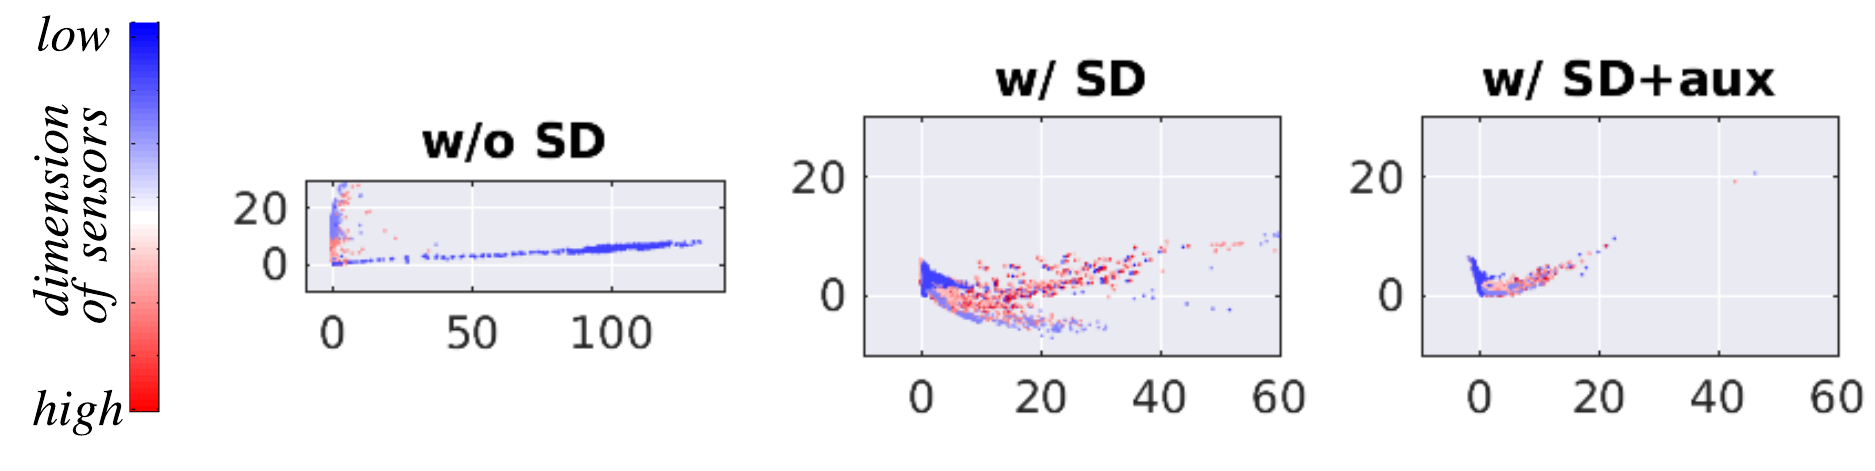
\includegraphics[width=0.8\columnwidth]{./MultimodalDRL/fig/pca.png}}
    \caption{Two-dimensional PCA embedding of the representations in the last hidden layer assigned by the policy networks.}
    \label{fig:aux_pca}
    % \vskip -0.2in
    \end{center}
\end{figure} 

\begin{figure}[t]
    \begin{center}
        \centerline{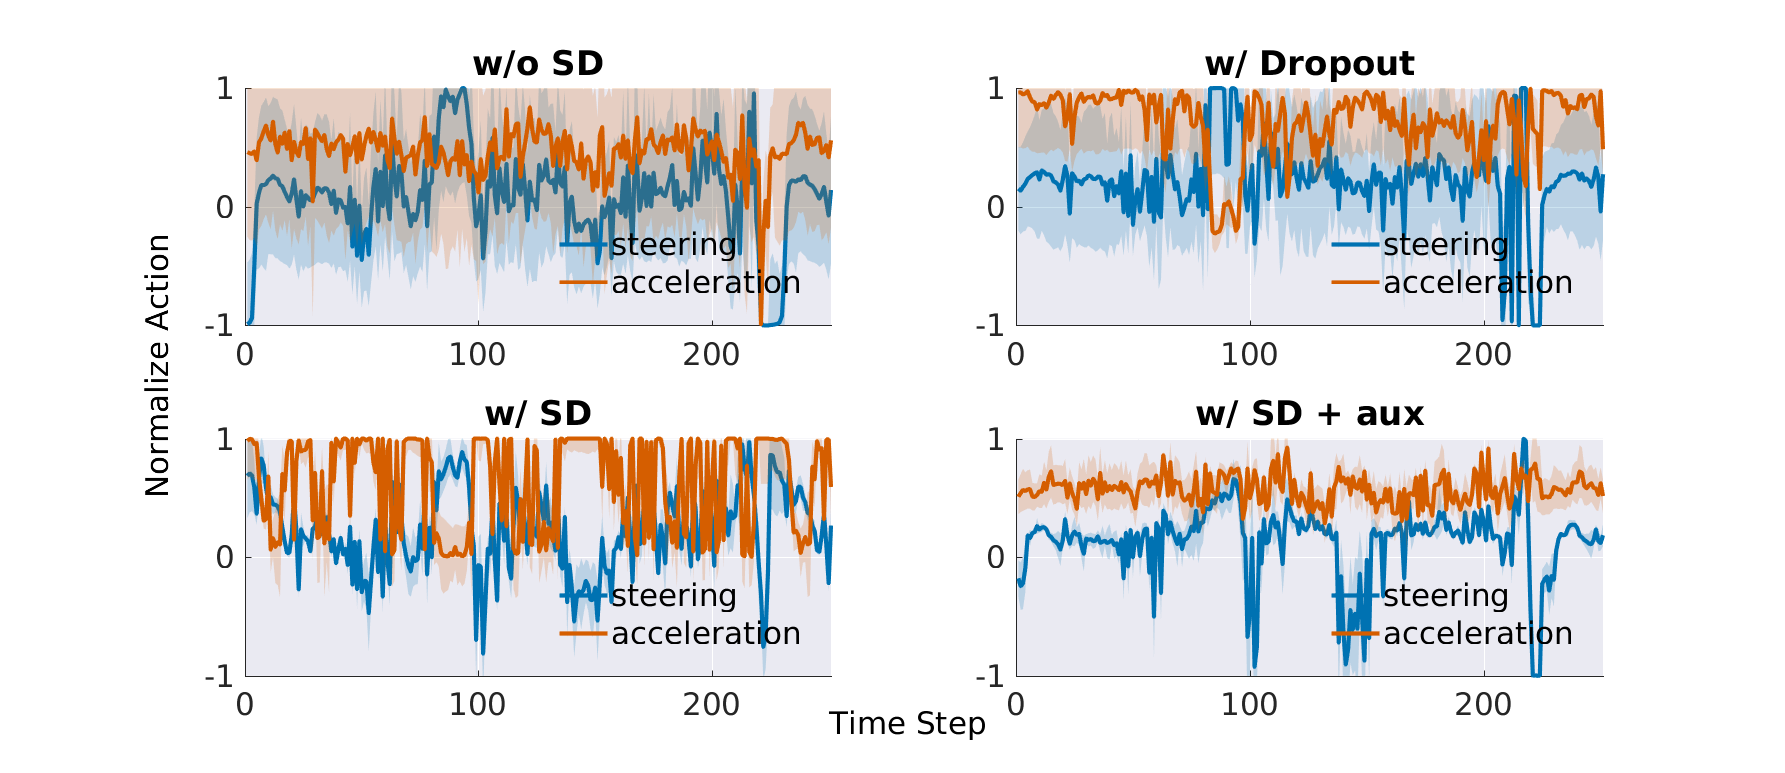
\includegraphics[width=\columnwidth]{./MultimodalDRL/fig/action_profile}}
        \caption{The variance of all the actions induced by sub-policy under each multimodal sensor policy. \textit{Upper-left}: naive policy without any regularization. \textit{Upper-right}: with standard Dropout. \textit{Lower-left}: with Sensor Dropout. \textit{Lower-right}: with Sensor Dropout and auxiliary loss.}
        \label{fig:action-profile}
    \end{center}
\end{figure} 

% \textbf{Effect of Auxiliary Loss:}
In this experiment we verify how the auxiliary loss helps reshape the multimodal sensor policy and reduce the action variance. 
We extract the representations of the last hidden layer assigned by the policy network throughout an fixed episode. At every time step, the representation induced by each sensor combination is collected. 
Our intuition is that the latent space represents how the policy network interprets the incoming sensor stream for reaction. Based on this assumption, an ideal multimodal sensor policy should map different sensor streams to an similar distribution as long as the information provided by each combination is representative to lead to the same output.

Fig. \ref{fig:aux_pca} shows the two-dimensional Principle Component Analysis (PCA) embedding on the latent space of each sub-policy. The blue dots correspond to the representations induced by the sub-policy that use high dimensional sensor (e.g. vision) as its input. On the other hand, the red dots represent the one with lower sensor stream such as odometry and range finder. Note that in practice, the covariance of the first third principle components contain around $85\%$. We provide the actual covariances for each component in the supplementary material.

As shown in Fig. \ref{fig:aux_pca}, the naive multimodal sensor policy has a scattered distribution over the latent space, indicating that representative information from each sensor is treated very differently. In comparison, the policy trained with SD has a concentrated distribution, yet it is still distinguishable w.r.t. different sensors. Adding the auxiliary training loss encourages the true sensor fusion as the distribution becomes more integrated. During training, the policy is not only forced to explicitly make decisions under each sensor combination, but also penalized with the disagreements among multimodal sensor policies. In fact, as shown in Fig. \ref{fig:action-profile}, the concentration of the latent space directly affect the action variance induced by each sub-policy. We provide the action variance value in the supplementary material.


\section{Discussion} \label{sec:mdrl-discussion}


\subsection{Full Sub-Policy Analysis}
\label{SD-full-config}

\begin{figure}[t]
\vskip -0.1in
\centering
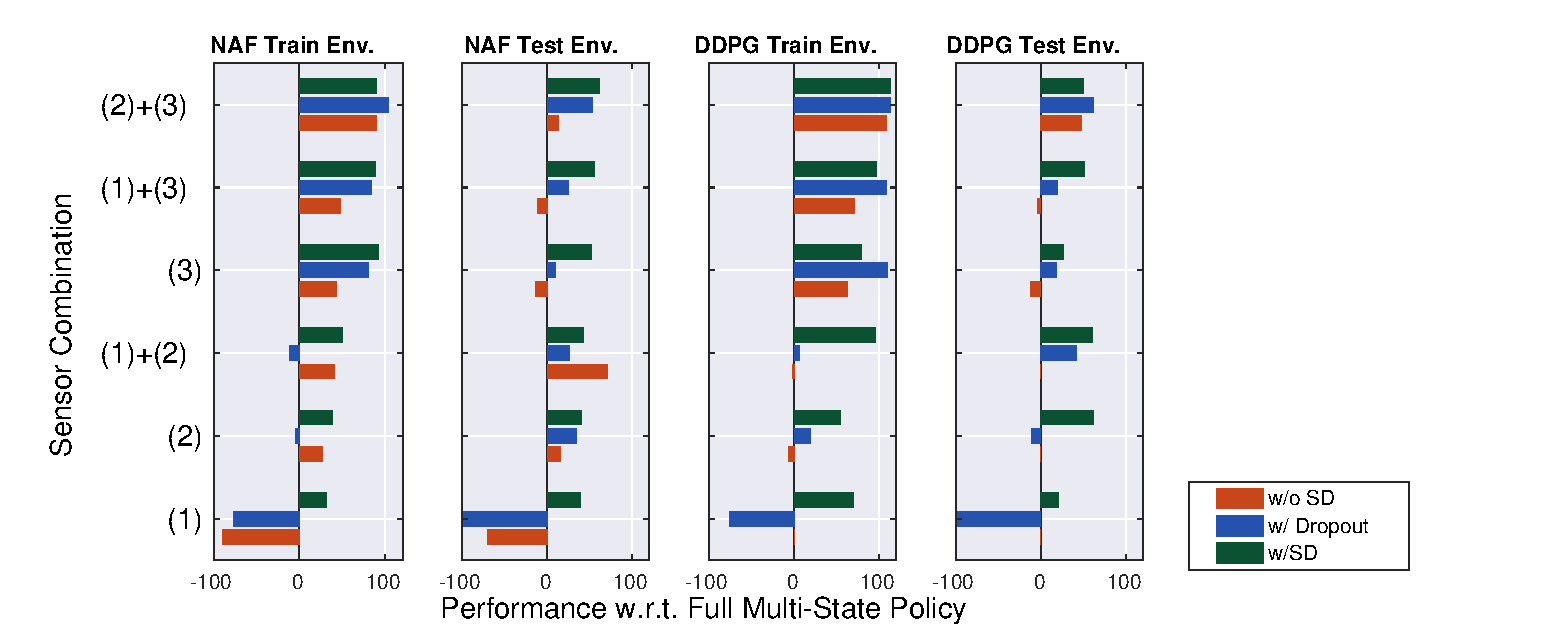
\includegraphics[width=\columnwidth]{./MultimodalDRL/fig/all_policy}
\caption{The full analysis of the performance of the total $6$ sub-policies. The (1), (2), and (3) labels in y-axis represent physical state, laser, and image, respectively. The x-axis represent the remaining performance w.r.t. the SD policy with all sensor, i.e. (1)+(2)+(3).}
\label{fig:full-sd-policy}
\vskip -0.1in
\end{figure} 

% \textbf{Full Sub-Policy Analysis: }
The performance of each sub-policy is summarized in Fig. \ref{fig:full-sd-policy}. 
As shown in the first and third column, the performance of the naive multimodal sensor policy (red) and the policy trained with standard Dropout (blue) drop dramatically as the policies lose access to image, which share $87.9\%$ of the total multimodal state. Though Dropout increases the performance of the policy in the testing environment, the generalization is limited to using full multimodel state  as input. On the other hand, Sensor Dropout (SD) generalize the policy across \textit{sensor module} that make the sub-policies successfully transfer to the testing environment. It is worth mentioning that the policies trained with SD is capable to operate when both laser and image sensor are blocked.

% less sensitive to the sensor dimensionality. 
% Note that in this experiment, the physical state, laser, and image share the portions of $1.7\%$, $10.3\%$, and $87.9\%$ of the total multimodal state. 

\subsection{Visualize Policy Attention Region}

\begin{figure}[t]
    \centering
    \begin{subfigure}[b]{0.48\linewidth}
        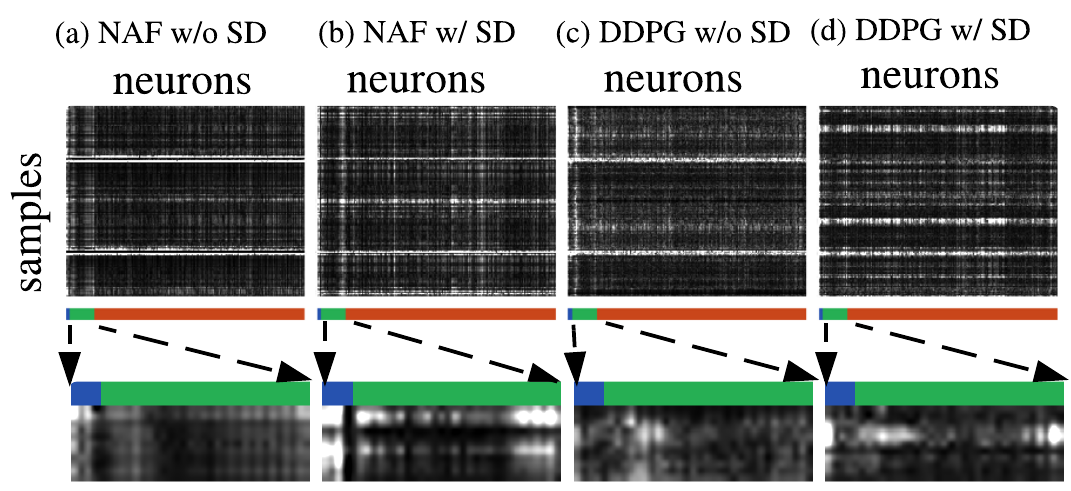
\includegraphics[width=\columnwidth]{./MultimodalDRL/fig/grad2_crop.png}
        \subcaption{}
        \label{fig:grad_exp}
    \end{subfigure}
    \begin{subfigure}[b]{0.48\linewidth}
        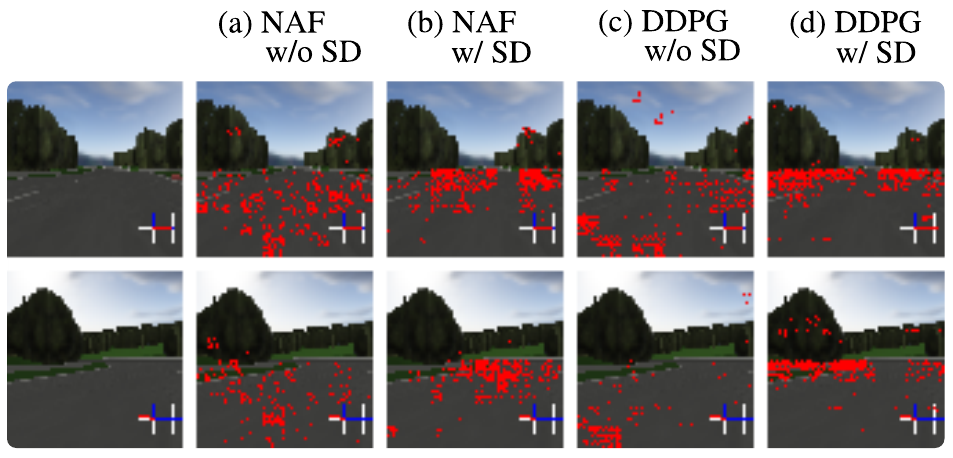
\includegraphics[width=\columnwidth]{./MultimodalDRL/fig/grad_image_new.png}
        \subcaption{}
        \label{fig:grad_exp_img}
    \end{subfigure}
    \caption{(a)The visualization of the magnitude of gradient for each neuron. The whiter color means the higher gradient. The color bar represents three different sensor modules: physical state(blue), Laser(green), and Image(red). (b) The gradient responses of actions on the image input for each of the multi-modal agents. The top $20\%$ gradients are marked red.}
    \label{fig:grad_exp_all}
\end{figure}

% \textbf{Visualize Policy Attention Region: }
The average gradient in the policy sensitivity section can also be used to visualize the region among each sensor that the policy network pays attention to. As shown in Fig. \ref{fig:grad_exp}, we observe that polices trained with SD have higher gradients on neurons corresponding to the corner inputs of the laser sensor, indicating that a more sparse and meaningful policy is learned. These corner inputs corresponded to the laser beams that are oriented perpendicularly to the vehicle's direction of motion, and give an estimate of its relative position on the track. To look for similar patterns, in Fig. \ref{fig:grad_exp_img}, image pixels with higher gradients are marked to visualize and interpret the policy's view of the world. We pick two scenarios, 1) straight track and 2) sharp left turn, depicted by the first and second rows in the figure. Note that though policies trained without SD tend to focus more on the road, those areas are in plain color and offer little salient information. In conclusion, policies trained with SD are more sensitive to features such as road boundary, which is crucial for long horizon planning. In comparison, network trained without SD has a relatively low and unclear gradients over both laser and image sensor state space.


% \subsection{Fusion Layer Configurations} \label{sec:SD-config}

% %%% Setting of SD used in this work %%%

% %%% talk more about some detailed in SD compared with Dropout %%%
% % 1. training speed (Fast: 0.5 > 0.4 > 0.25 )
% % 2. performance in both training/testing (Higher: 0.5 < 0.4 < 0.25 )
% % 3. Individual policy (Higher: 0.5 < 0.4 < 0.25 )
% Following the notations used in Section \ref{sec:SD-implement}, we observe that as the probabilities $p_1,~p_2$ increase, the policy convergence rate and the normalized average rewards induced by each sensor subset also increase, as described in Section \ref{sec:policy}. However, the performance of the full policy decreases in both training and testing environment. This empirical result suggests a more principled way to apply Sensor Dropout. For instance, we can start with a high value for $(p_1,~p_2)$ and benefit from faster policy convergence for each sensor subset and then gradually decrease the probability to promote fusion. 

% \newpage

\section{Supplementary Material}

% \appendix


\begin{table}[t]
    \vskip 0.1in
    \caption{Covariance of the first three Principle Component}
    \label{table:pca-3-covariance}
    \vskip 0.1in
    \centering
    \begin{small}
    \begin{sc}
    \begin{tabular}{c|ccc|ccc}
    \toprule 
    \centering
     & \multicolumn{3}{c}{NAF} & \multicolumn{3}{c}{DDPG}  \\
     Principle Component & w/oSD & w/SD & w/SD+aux & w/oSD & w/SD & w/SD+aux \\ \midrule \midrule
     First (\%) & 94.9  &  82.0  &  58.9 & 
                93.4  &  59.2  &  47.4 \\
     Second  (\%) & 4.1  &  12.3  &  25.2 & 
                    3.1  &  20.7  &  21.9 \\ 
    Third  (\%) & 0.6  &  3.1  &  5.3 & 
                1.6  &  6.2  &  6.1 \\ \toprule
    \end{tabular}
    \end{sc}
    \end{small}
\end{table}

\begin{table}[t]
    \vskip 0.1in
    \caption{Action Variation w.r.t. multimodal sensor}
    \label{table:pca-action-variance}
    \vskip 0.1in
    \centering
    \begin{small}
    \begin{sc}
    \begin{tabular}{c|ccc|ccc}
    \toprule 
    \centering
     & \multicolumn{3}{c}{NAF} & \multicolumn{3}{c}{DDPG}  \\
     & w/oSD & w/SD & w/SD+aux & w/oSD & w/SD & w/SD+aux \\ \midrule \midrule
     Steering & 0.1177  &  0.0819  &  \textbf{0.0135} & 
                0.3329  &  0.0302  &  \textbf{0.0290} \\
     Acceleration & 0.4559  &  0.0472  &  \textbf{0.0186} & 
                    0.5714  &  0.0427  &  \textbf{0.0143} \\ \toprule
    \end{tabular}
    \end{sc}
    \end{small}
\end{table}

The covariance of PCA and the actual action variance is summarized in Table \ref{table:pca-3-covariance} and \ref{table:pca-action-variance}, respectively.


\end{document}